\documentclass[12pt, twoside]{article}
\usepackage[letterpaper, margin=1in, headsep=0.5in]{geometry}
\usepackage[english]{babel}
\usepackage[utf8]{inputenc}
\usepackage{amsmath}
\usepackage{amsfonts}
\usepackage{amssymb}
\usepackage{tikz}
\usetikzlibrary{quotes, angles}
\usepackage{graphicx}
\usepackage{enumitem}
\usepackage{multicol}

\newif\ifmeta
\metatrue %print standards and topics tags

\title{Regents Geometry}
\author{Chris Huson}
\date{September 2020}

\usepackage{fancyhdr}
\pagestyle{fancy}
\fancyhf{}
\renewcommand{\headrulewidth}{0pt} % disable the underline of the header
\raggedbottom


\fancyhead[LE]{\thepage}
\fancyhead[RO]{\thepage \\ Name: \hspace{4cm} \,\\}
\fancyhead[LO]{BECA / Dr. Huson / Geometry 07-Similarity\\* pset ID: 105}

\begin{document}

\subsubsection*{7-2bDN-Graphing-practice}
\begin{enumerate}
\item \begin{enumerate}
    \item Graph and label the two equations. Mark their intersection as an ordered pair.
      \begin{multicols}{2}
        $y =-\frac{3}{2}x-7$ \\
        $2x-3y=-18$ \hfill (4 pts)
      \end{multicols}     \vspace{1.5cm}
    \item Find the slopes of the two lines. \hfill (2 points)
      \begin{multicols}{2}
        $m_1=$ \\
        $m_2=$
      \end{multicols}
    \item Are the lines parallel, perpendicular, or neither? Justify your answer with an equation or inequality using the slopes. \hfill (2 points)
    \vspace{1.5cm}
  \end{enumerate}
    \begin{center}
      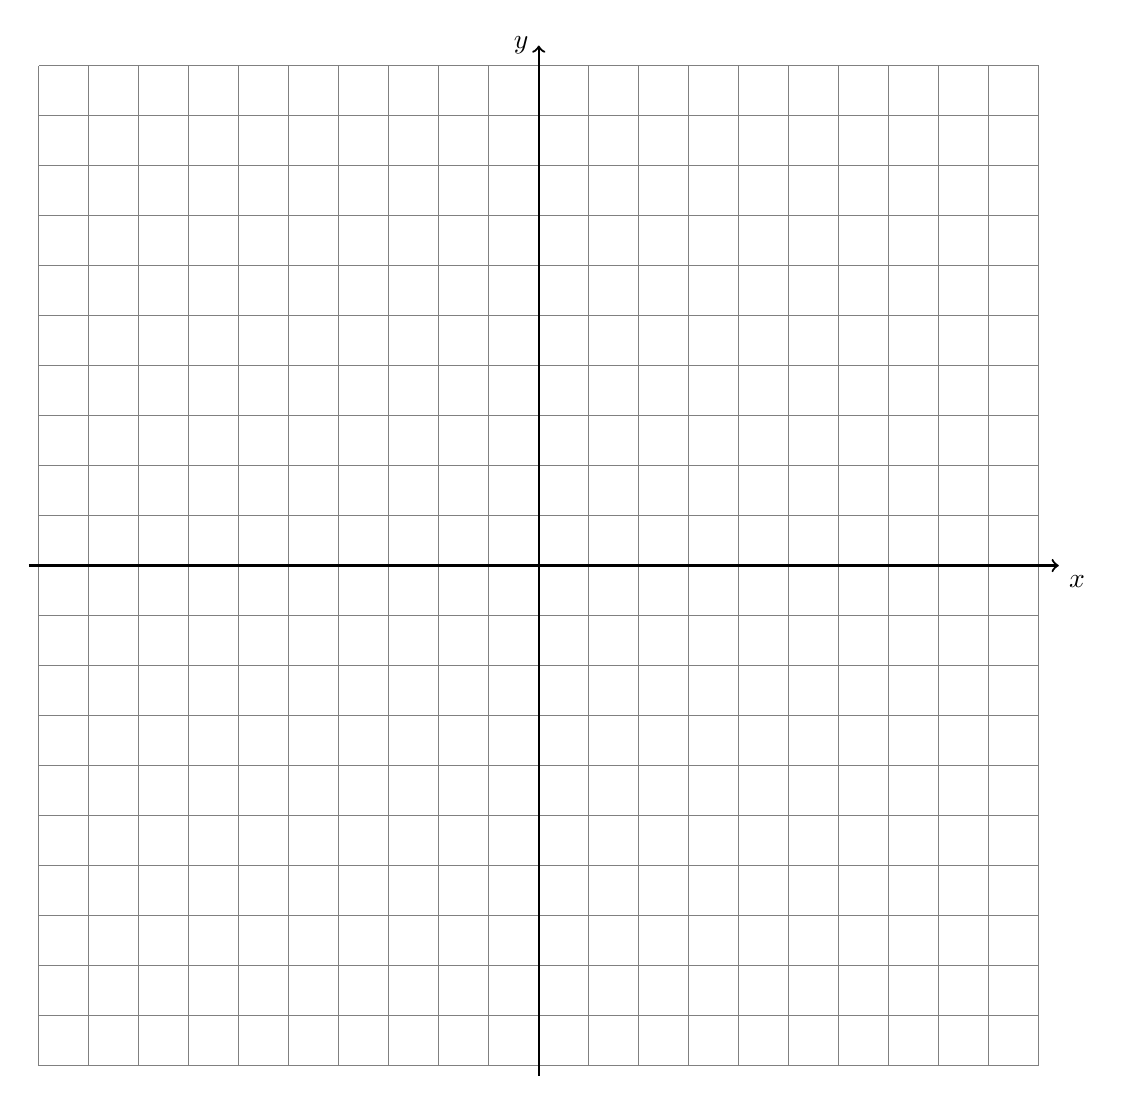
\begin{tikzpicture}[scale=.635]
        \draw [help lines] (-10,-10) grid (10,10);
        \draw [thick, ->] (-10.2,0) -- (10.4,0) node [below right] {$x$};
        \draw [thick, ->] (0,-10.2)--(0,10.4) node [left] {$y$};
      \end{tikzpicture}
    \end{center}

  \newpage
\item A dilation centered at $A$ maps $\triangle ABC \rightarrow \triangle ADE$. Given the sides of the preimage, $AC = 6$, $BC = 4$, $AB = 8$, and of $DE = 14$ find the scale factor $k$ and the lengths $AD$ and $AE$. Then find $CE$ and $BD$. \vspace{1cm}
  \begin{multicols}{2}
    \begin{enumerate}
      \item $k=$ \vspace{0.3cm}
      \item $AD=$ \vspace{0.3cm}
      \item $AE=$ \vspace{0.3cm}
      \item $CE=$
      \item $BD=$
    \end{enumerate}
    \begin{flushright}
      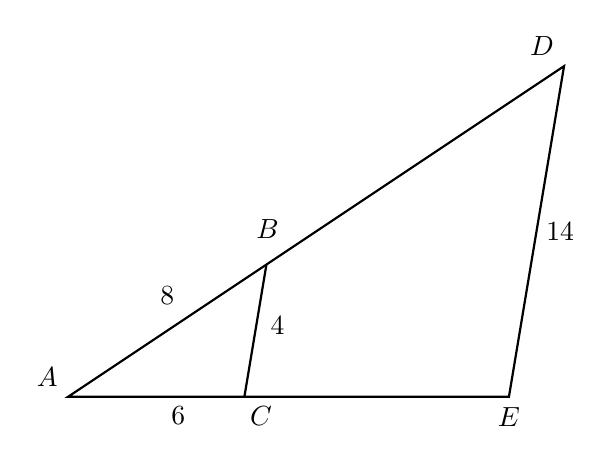
\begin{tikzpicture}[scale=0.7]
        \draw [-, thick] (0,0) node[above left]{$A$}--
        (8,0) node[below]{$E$}--
        (9,6) node[above left]{$D$}--cycle;
        \draw [thick] (3.2,0)--(3.6,2.4);
        \node at (3.5,0) [below]{$C$};
        \node at (4,2.7) [above left]{$B$};
        \node at (2, 0) [below]{$6$};
        \node at (1.8,1.5) [above]{$8$};
        \node at (8.5, 3) [right]{$14$};
        \node at (3.5, 1.3) [right]{$4$}; \vspace{1cm}
      \end{tikzpicture}
    \end{flushright} 
  \end{multicols}\vspace{1.5cm}

\item Given $\triangle ABP \sim \triangle JKP$ as shown below. $AB=5.7$, $AP=7.4$, $BP=3.6$, and $KP=9.0$. Find $JK$.
  \begin{flushright}
  \begin{tikzpicture}[scale=1.4]
      \draw [thick]
        (-0.25,-1)node[below left]{$B$}--
        (0.5,2)node[left]{$K$}--
        (4,0)node[below left]{$J$}--
        (0,0)node[above left]{$P$}--
        (-2,0)node[left]{$A$}--cycle;
    \end{tikzpicture}
    \end{flushright}
    \vspace{2cm}

\newpage
\item $A(-1,-1)$ is one endpoint of $\overline{AB}$. The segment's midpoint is $M(3,1)$, as shown below.  
  \begin{multicols}{2}
    \begin{enumerate}
    \item What translation maps \\[0.25cm] $A(-1,-1) \rightarrow M(3,1)$?
    \item Find the other endpoint, $B$. \vspace{2cm}
    \end{enumerate}
    \begin{flushright}
      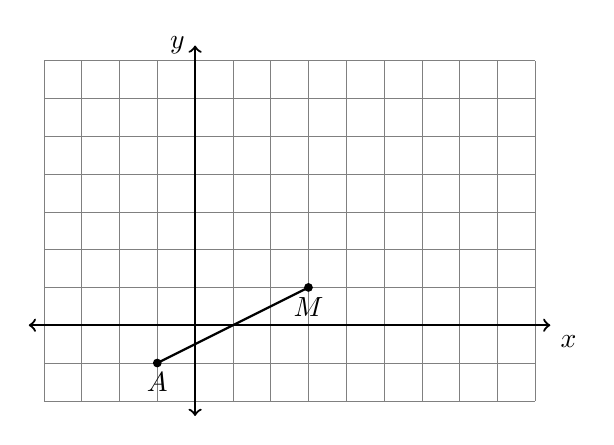
\begin{tikzpicture}[scale=.48]
        \draw [help lines] (-4,-2) grid (9,7);
        \draw [thick, <->] (-4.4,0) -- (9.4,0) node [below right] {$x$};
        \draw [thick, <->] (0,-2.4)--(0,7.4) node [left] {$y$};
        \draw [thick] (-1,-1)--(3,1);
        \draw [fill] (-1,-1) circle [radius=0.1] node[below] {$A$};
        \draw [fill] (3,1) circle [radius=0.1] node[below] {$M$};
      \end{tikzpicture}
    \end{flushright}
  \end{multicols}

\item In the diagram below, $\overline{AD}$ has endpoints with coordinates $A(-3,1)$ and $D(6,-2)$. What points $B$ and $C$ trisect $\overline{AD}$ into three congruent segments? Mark and label them on the graph. State their coordinates.
    \begin{flushright}
      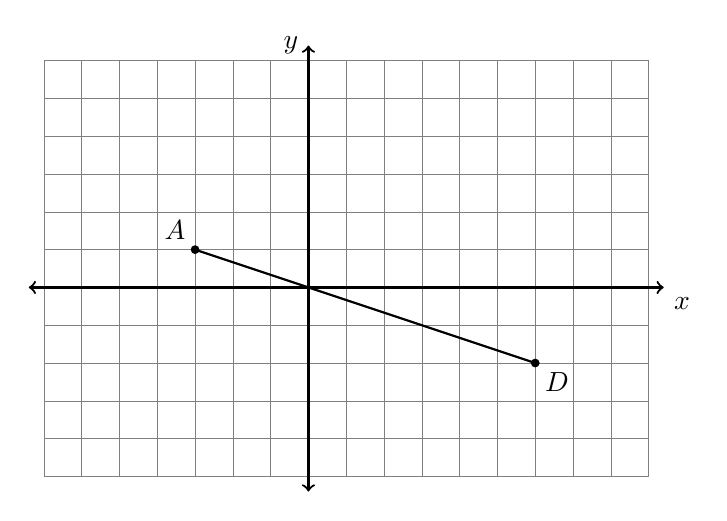
\begin{tikzpicture}[scale=.48]
        \draw [help lines] (-7,-5) grid (9,6);
        \draw [thick, <->] (-7.4,0) -- (9.4,0) node [below right] {$x$};
        \draw [thick, <->] (0,-5.4)--(0,6.4) node [left] {$y$};
        \draw [thick] (-3,1)--(6,-2);
        \draw [fill] (-3,1) circle [radius=0.1] node[above left] {$A$};
        \draw [fill] (6,-2) circle [radius=0.1] node[below right] {$D$};
      \end{tikzpicture}
    \end{flushright}
\item Given $\triangle ABC$ is isosceles but not equilateral with $\angle A \cong \angle C$. \hfill (\emph{not draw to scale})
    \begin{enumerate}
    \item Mark the congruent sides \& angles of $\triangle ABC$. \\[0.25cm]
    Circle True or False:
    \begin{multicols}{2}
    \item True \quad False \quad $\overline{AB} \cong \overline{BC}$
    \item True \quad False \quad $\overline{AB} \cong \overline{AC}$
    \item True \quad False \quad $\overline{BC} \cong \overline{AC}$
    \begin{flushright}
    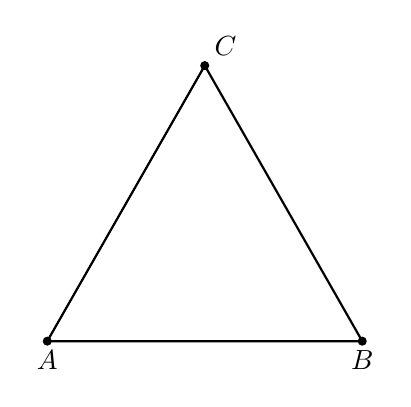
\begin{tikzpicture}[scale=1]
      \draw [thick](0,0)--(4,0)--(2,3.5)--(0,0);
      \draw [fill] (0,0) circle [radius=0.05] node[below]{$A$};
      \draw [fill] (4,0) circle [radius=0.05] node[below]{$B$};
      \draw [fill] (2,3.5) circle [radius=0.05] node[above right]{$C$};
    \end{tikzpicture}
    \end{flushright}
  \end{multicols}
  \end{enumerate}
  %\vspace{1cm}

  \newpage
\item Given isosceles $\triangle ABC$ with $\overline{AB} \cong \overline{AC}$. \hfill (\emph{the diagram is not to scale})
    \begin{enumerate}
      \item Mark the congruent sides \& angles of $\triangle ABC$. \\[0.25cm]
      Circle True or False:
      \begin{multicols}{2}
      \item True \quad False \quad $\angle A \cong \angle B$
      \item True \quad False \quad $\angle A \cong \angle C$
      \item True \quad False \quad $\angle B \cong \angle C$
      \item T \quad F \quad $m\angle A + m\angle B + m\angle C =180$   
      \begin{flushright}
      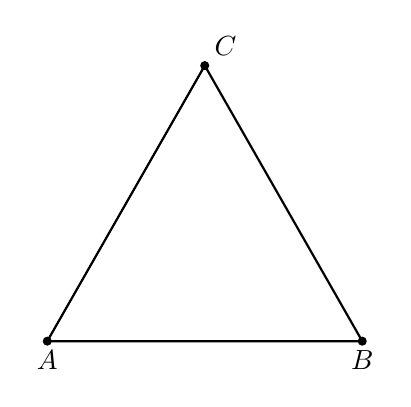
\begin{tikzpicture}[scale=1]
        \draw [thick](0,0)--(4,0)--(2,3.5)--(0,0);
        \draw [fill] (0,0) circle [radius=0.05] node[below]{$A$};
        \draw [fill] (4,0) circle [radius=0.05] node[below]{$B$};
        \draw [fill] (2,3.5) circle [radius=0.05] node[above right]{$C$};
      \end{tikzpicture}
      \end{flushright}
    \end{multicols}
    \end{enumerate}
      \vspace{1cm}
  
\item Given isosceles $\triangle RSU$ with $\overline{RS} \cong \overline{SU}$. \hfill (\emph{the diagram is not to scale})
      \begin{enumerate}
      \item Mark the congruent sides \& angles of $\triangle RSU$. %\\[0.25cm]
        \begin{multicols}{2}
          Circle True or False:
        \item True \quad False \quad $\angle R \cong \angle RSU$
        \item True \quad False \quad $\angle R \cong \angle U$
        \item True \quad False \quad $\angle RSU \cong \angle U$
        \item True \quad False \quad $\angle R \cong \angle TSU$
        \begin{flushright}
        \begin{tikzpicture}[scale=1.1]
          \draw [<-, thick] (7,0)--
          (6.5,0) node[below]{$T$}--
          (0.8,0) node[below]{$R$}--
          (3,3.1) node[above]{$U$}--
          (5,0) node[below]{$S$};
        \end{tikzpicture}
        \end{flushright}
      \end{multicols}
        \item True \quad False \quad $\angle RSU \cong \angle TSU$
        \item True \quad False \quad $m\angle RSU + m\angle TSU =180$  
        \item True \quad False \quad $m\angle R + m\angle RSU + m\angle U =180$   
    \end{enumerate}

\newpage
\subsubsection*{7.2 Spicy: Similar triangles, dilations}

\item The diagram below shows $\triangle ABC \sim \triangle ADE$, with $\overline{AEB}$, $\overline{ADC}$, and $\angle ACB \cong \angle AED$. $AB=8$, $AD=4$, and $DE=2$.
  \begin{multicols}{2}
    \begin{enumerate}
      \item $\triangle ADE \rightarrow$ \rule{2cm}{0.15mm} \vspace{1cm}
      \item $\overline{AD} \rightarrow$ \rule{2cm}{0.15mm} \vspace{1cm}
      \item What is the scale factor?\\[0.5cm] $k=$  \rule{2cm}{0.15mm}
      \item What is the length of $\overline{BC}$?
    \end{enumerate}
      \begin{tikzpicture}[scale=1.3]
        \draw [thick]
        (0,0) node[above right] {$A$}--
        (230:6) node[below left] {$B$}--
        (260:4.75) node[below right] {$C$}--cycle;
        \draw [thick]
        (230:2.375) node[above left] {$E$}--
        (260:3) node[right] {$D$}--cycle;
      \end{tikzpicture}
    \end{multicols} \vspace{2cm}
    
\item Given $\triangle ABC \sim \triangle ADE$ with sides $AC = 9$, $BC = 6$, $AB = 12$, and of $DE = 10$ find the scale factor $k$ and the lengths $AD$ and $AE$. Then find $CD$. \vspace{1cm}
  \begin{multicols}{2}
    \begin{enumerate}
      \item $k=$ \vspace{1cm}
      \item $AD=$ \vspace{1cm}
      \item $AE=$ \vspace{1cm}
      \item $CD=$
    \end{enumerate}
    \begin{flushright}
      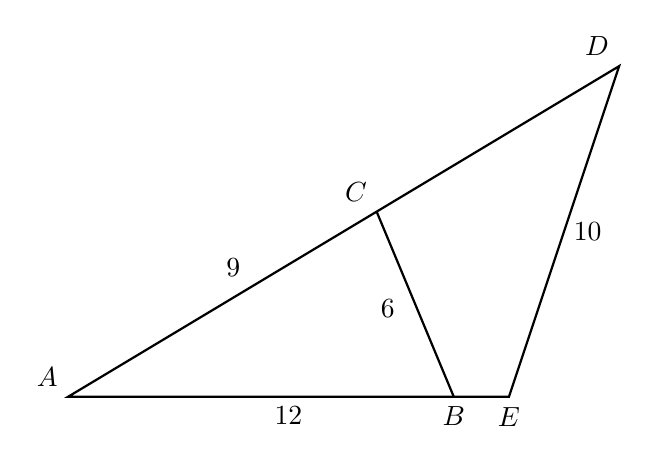
\begin{tikzpicture}[scale=0.7]
        \draw [-, thick] (0,0) node[above left]{$A$}--
        (8,0) node[below]{$E$}--
        (10,6) node[above left]{$D$}--cycle;
        \draw [thick] (7,0)--(5.6,3.36);
        \node at (7,0) [below]{$B$};
        \node at (5.6,3.36) [above left]{$C$};
        \node at (4, 0) [below]{$12$};
        \node at (3,2) [above]{$9$};
        \node at (9, 3) [right]{$10$};
        \node at (5.5, 1.6) [right]{$6$}; \vspace{1cm}
      \end{tikzpicture}
    \end{flushright} 
  \end{multicols}\vspace{1.5cm}

\end{enumerate}
\end{document}